% Comando para definir la clase de documento: artículo (article), libro (book), etc. 
\documentclass{article}

\usepackage{courier}

\usepackage{lmodern}

% Comando para usar el paquete geometry y definir el tamaño del papel, el tamaño de los márgenes, etc.
\usepackage[a4paper,margin=3cm]{geometry}

% Comando para definir el interlineado 1.25
\linespread{1.5} 

% Comando para usar caracteres con codificacion UTF-8
\usepackage[utf8]{inputenc}

% Comando para usar el paquete babel en español (por ejemplo: Resumen, no Abstract)
\usepackage[spanish,es-tabla]{babel}

% Comando para usar el paquete textgreek y poder insertar letras griegas en modo texto
\usepackage{textgreek}

% Comando para usar el paquete graphicx y así poder incluir figuras
\usepackage{graphicx}

% Comando para usar el paquete float y así posicionar las figuras con el argumento H
\usepackage{float}

% Comando para usar el paquete authblk y así poder incluir la institución del autor
\usepackage{authblk}

% Comando para usar el paquete tocloft y así poder cambiar la tabla de contenidos, etc. 
\usepackage{tocloft}

% Comando para usar puntos como separadores en la tabla de contenidos, etc. 
\renewcommand{\cftsecleader}{\cftdotfill{\cftdotsep}}

% Comando para usar el paquete parskip y definir el espaciado entre párrafos y su indentado
\usepackage[skip=6pt plus 1pt,tocskip=3pt,indent=1cm]{parskip}

% Comando para usar los paquetes amsmath y amssymb, y así poder incluir fórmulas matemáticas
\usepackage{amsmath,amssymb}

% Comando para usar el paquete xcolor y así poder personalizar los colores
\usepackage{xcolor}

% Comando para definir un nuevo color
\definecolor{gris}{RGB}{240,240,240}

% Comando para usar el paquete listings y así poder mostrar código de LaTeX dentro del texto
\usepackage{listings}

% Comando para permitir la división del código de LaTeX presente dentro del texto
\lstset{basicstyle=\ttfamily\normalsize,breaklines=true}

% Comando para usar el paquete minted y así emplear resaltado de sintaxis de código fuente
\usepackage[newfloat]{minted}

% Comando para usar el paquete mdframed y así poder poner fondo y borde con minted
\usepackage{mdframed}

% Comando para usar el paquete caption y así poder poner títulos estilo APA 7 
\usepackage[labelfont=bf,textfont=it,labelsep=newline,justification=justified,singlelinecheck=off,position=top,skip=6pt]{caption}

% Comando para usar el paquete subcaption y así poder poner notas estilo APA 7 
\usepackage[textfont=normalfont,justification=justified,singlelinecheck=off,position=bottom,skip=6pt]{subcaption}

% Comando para cambiar el interlineado en los títulos estilo APA 7 de figuras y tablas 
\captionsetup{font={stretch=1.5}}

% Comando para cambiar a 6pt (+3pt/-2pt) el espacio antes de las figuras
\setlength{\belowcaptionskip}{6pt plus 3pt minus 2pt}

% Comando para usar el paquete array y así poder alinear el contenido en las tablas
\usepackage{array}

% Comando para usar el paquete multirow y así tener celdas de más de una fila en tablas
\usepackage{multirow}

% Comando para cambiar la altura de las filas en la tablas 
\renewcommand\arraystretch{1.5}

% Comando para usar el paquete csquotes y así automatizar la inserción de citas 
\usepackage[autostyle,spanish=mexican,thresholdtype=words,threshold=39,csdisplay=true]{csquotes}

% Comando para cambiar el indentado de las citas largas 
\renewenvironment{quote}{\list{}{\leftmargin=1.5cm\rightmargin=0cm}\item\relax}{\endlist}

\renewenvironment{abstract}{\list{}{\leftmargin=1.5cm\rightmargin=0cm}\item\relax}{\endlist}

\renewenvironment{keyword}{\list{}{\leftmargin=1.5cm\rightmargin=0cm}\item\relax}{\endlist}

% Comando para usar el paquete biblatex y así poder administrar fuentes bibliográficas
\usepackage[backend=biber,style=apa]{biblatex}

% Comando para que biblatex funcione en español
\DeclareLanguageMapping{spanish}{spanish-apa}

% Comando para importar una bibliografía y así poder usarla con biblatex
\addbibresource{latex.bib}

% Comando para definir el comando keywords (solo si este no existe previamente)
\providecommand{\keywords}[1]{\par\bigskip\noindent\textit{Palabras clave:} #1}

\begin{document}
    % Comando para definir el título del documento
    \begin{center}
        {\fontsize{24pt}{24pt}\selectfont La balanza electrónica como periférico de PC} 

        %SALTO DE LINEA%
        \hspace{1.5cm}
        
        % Comando para definir al autor o a los autores del documento
        {Juan Ignacio Szapiro}

        \fontsize{9pt}{9pt}\texttt{juanignacioszapiro@gmail.com}

        \fontsize{10pt}{10pt}\textit{Instituto Nacional Superior del Profesorado Técnico, Ciudad Autónoma de Buenos Aires, Argentina}
        
        %SALTO DE LINEA%
        \hspace{1.5cm}
    \end{center}
    
   
    \renewcommand{\abstractname}{\vspace{-\baselineskip}}
    \begin{abstract}\noindent{
    El presente texto informativo surge en base a las pautas establecidas en la carrera Informática Aplicada de UTN-INSPT, materia Sistemas de Computación I, dictada por el Profesor Diego Corsi. En el mismo se abarca información general de la balanza electrónica como periférico de PC, considerando su definición, tipos de conexión, diferentes softwares, etc. con el fin de generar una recopilación de datos a falta de la existencia previa de uno.}

    %SALTO DE LINEA%
    \hspace{1.5cm}
    \end{abstract}
    
    \begin{keyword}
    \fontsize{10pt}{10pt}{\textit{Palabras clave:} balanza electrónica, balanza digital, conexión, datos.}
    \end{keyword}
    
    \section{Definición}
        {\noindent {FEMTO (s.f.) define la balanza electrónica como:} }
        \begin{quote}
        Son instrumentos de pesaje de funcionamiento no automático que utilizan la acción de la gravedad para determinación de la masa. Se compone de un único receptor de carga (plato) donde se deposita el objeto para medir. Una célula de carga de carga (SIC) mide la masa a partir de la fuerza (peso) ejercida por el cuerpo sobre el receptor de carga. El resultado de
        esa medición (indicación) aparecerá reflejado en un dispositivo indicador.
        \end{quote}

    \section{Funcionamiento interno de balanzas electrónicas}
        {\noindent {La transferencia de información es a través de señales eléctricas que se generan, muy resumidamente,
        transformando la fuerza del peso a través de un medidor de tensión, un dispositivo que se usa para
        medir la tensión de un objeto, y un sensor de celda de carga (Figura 1), un dispositivo electrónico que
        se usa para convertir una fuerza en una señal eléctrica.
        Cuando se coloca un artículo en la báscula, el peso primero se distribuye uniformemente. Debajo de
        la bandeja plana de una báscula digital se encuentran, por ejemplo, cuatro clavijas ligeramente
        elevadas en las esquinas que sirven para distribuir la fuerza del peso de manera uniforme. El
        mecanismo de la báscula digital aplica la fuerza del peso a un extremo de una celda de carga. A
        medida que se aplica el peso, ese extremo de la celda de carga se dobla hacia abajo.
        La fuerza de un peso deforma la galga extensiométrica. El medidor de tensión puede consistir en
        pistas de metal, o láminas, unidas a una placa de circuito impreso u otro respaldo. Cuando se tensa la
        hoja de metal, el respaldo se flexiona o se estira.}\\
        {El medidor de tensión luego convierte la deformación en una señal eléctrica. Debido a que la celda
        de carga tiene energía eléctrica, a medida que se mueve hacia abajo, la resistencia cambia. El pequeño
        cambio resultante en la resistencia se convierte en una señal eléctrica. La señal se ejecuta a través de
        un convertidor analógico a digital y luego pasa a través de un microchip que traduce los datos. Como
        resultado de este cálculo final, los números que indican el peso del objeto aparecen en la pantalla
        LCD de la báscula digital.
        (MARYNIA , K., s. f.).}}

        \begin{figure}[H]
        	\caption{Sensor de celda de carga}
            \begin{subfigure}{1.0\textwidth}
        	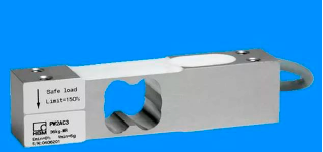
\includegraphics[width=0.65\textwidth]{Figura 1 - Sensor de celda de carga}
        	\subcaption*{\textit{Nota.} Adaptada de MARYNIA , K. (s. f.). How Does a Digital Scale Work? Hunker.}
            \end{subfigure}
        	\label{fig:miktex}
        \end{figure}
        \vspace{-2.0\baselineskip}

    \section{Tipos de conexión}
        {\noindent {Siempre y cuando se tenga instalado en la PC el software adecuado para la sincronización con la
        balanza, se pueden contar principalmente con dos tipos de conexión: alámbricos e inalámbricos. Los
        primeros siendo a través de conectores hembra de USB o RS-232 y los segundos Bluetooth o Wifi,
        esto siendo de manera no excluyente, por lo que una sola máquina podría tener todos los tipos de
        conexión mencionados, enviando y recibiendo información de datos binarios en cortas distancias. Así
        se agilizan procesos operativos tanto como administrativos. (Balanzas con Conexión a
        Computadoras., s. f.).}}
    \section{Algunos softwares para la PC y sus características}
        {\noindent {En esta sección se desarrollan tres tipos de software diferentes y sus características a modo de ejemplo
        y en orden alfabético.}
        
        \subsection{GALIL - Pesaje de camiones}
        {\noindent El software GALIL, para pesaje de camiones, transfiere de manera instantánea el peso y las
        indicaciones de movimiento y opera tanto con tara manual como con pesajes múltiples. Se tiene la
        capacidad de realizar el pesaje en balanzas cortas por pesadas aditivas, utilización de base de datos
        Compac Edition (.sdf) y opciones SQL Server, SQL Server Express o My SQL y la capacidad de
        almacenar camiones pendientes en las mismas, sistema de ticketera totalmente configurable por el
        usuario permitiendo editar y posicionar leyendas y campos de datos, para formularios pre-impresos
        u hojas en blanco y siempre operando acorde a la resolución del AFIP, siendo compatible con
        cualquier indicador con comunicación a PC e indicaciones de la línea SIPEL y por último, pero no
        menos importante tiene la posibilidad de realizar operaciones sencillas con ayuda en la pantalla.
        (www.sipel.com.ar, s. f.).}
        
        \subsection{LabX Balance Software}
        {\noindent Las siguientes características fueron aportadas por METTLER TOLEDO:}
        \begin{itemize}
        \item Flujo de datos integrado sin problemas
        \item Documentación automática
        \item Manejo central de la balanza
        \item Aumento de la eficiencia
        \end{itemize}
        
        \subsection{Software para balanzas EasyDirect}
        {\noindent Este software realiza operaciones de pesaje paralelo de hasta diez balanzas a través de conexiones de
        Ethernet o RS232, capacidad de generar informes simples y claros con exportación de manera manual
        o automática de los siguientes tipos de datos: XML, CSV, XLSX o PDF. Se logra reducción de errores
        de transcripción manual, consulta de datos con facilidad, ahorro tiempo y almacenado datos en forma
        segura. (M.-T. I. I. all rights. reserved, s. f.)}
        
    \section{Utilidades}
        {\noindent El uso más común en la vida cotidiana es la balanza gramera que se encuentra en diferentes comercios
        con el fin de calcular el precio por peso de los diferentes productos, la balanza contadora con
        funcionamiento de cálculo de piezas, la balanza etiquetadora permite imprimir y programar el
        contenido a impresión. Dentro del sector industrial se utilizan para mantener de manera controlada el
        inventario pesando con exactitud los grandes volúmenes de materia, para los cuales se requiere
        básculas con estructuras robustas. Estas últimas también se pueden encontrar en zonas de control
        vehicular sirviendo, por ejemplo, para mantener por debajo, del peso límite permitido por las
        autoridades, a los camiones de transporte en autopistas y carreteras. Las balanzas de laboratorio entran
        4 en la categoría de balanzas de precisión y analíticas que permiten obtener un resultado sumamente
        preciso. (Tipos de balanzas Electrónicas o Digitales, s. f.)}
        
    \section{Métodos para obtener el peso de un vehículo}
        {\noindent Existen tres tipos de medición de peso de un vehículo:}
        \begin{itemize}
        \item Un eje: el método más engorroso, un camión avanza gradualmente a través de una sola
        báscula, deteniéndose cada vez que un juego de ruedas está en la báscula. Una vez pesados
        todos los ejes, se suma el total.
        \item Cuando para: se utiliza una serie de básculas para que se pueda pesar todo el camión a la
        vez. Las básculas suelen estar conectadas a un solo controlador electrónico que combina
        automáticamente los pesos por eje para obtener el peso bruto.
        \item Pesaje en movimiento (PEM): un método que está cobrando impulso, PEM utiliza una serie
        de sensores integrados para calcular el peso por eje a medida que un camión pasa sobre la
        plataforma del sensor. A diferencia de los otros dos métodos, no es necesario que el camión
        se detenga por completo mientras está en la báscula. De hecho, algunos sistemas PEM se
        instalan en las autopistas para que todo el tráfico se controle a la velocidad.
        \end{itemize}
        (How do truck weigh stations work?, 2001, mayo 1)

    \section{Conclusión}
        {\noindent En la instancia de investigación para empezar la redacción de este proyecto me encontré con la falta
        de trabajos desarrollando las balanzas electrónicas con una existencia previa. Considerando esto y el
        extenso, pero poco abarcativo desarrollo de este artículo aún queda mucho por expandir sobre
        balanzas electrónicas como periféricos de PC.}

    \section{Referencias}
        %otra manera de citar
        %\citeurl{abc}
        %\citeauthor{abc}
        %\citeyear{abc}
        %\nocite[pp. 19-21]{abc}
        \nocite{BalanzasElectrónicasLima_BalanzasConConexiónAComputadoras}      \nocite{LasMejores10EmpresasDeBalanzas_BalanzasConConexiónAComputadoras}
        \nocite{FEMTO_BalanzaElectrónicaDePrecisión}
        \nocite{KOLAKM._HowDoesADigitalScaleWork?Hunker}
        \nocite{HowStuffWorks_HowDoTruckWeighStationsWork?}
        \nocite{M.T.I.I._SoftwareParaBalanzasEasyDirec}
        \nocite{METTLERTOLEDO_GroupMarComRITM692067LS}
        \nocite{BalanzasPrecisur_TiposDeBalanzasElectrónicasODigitales}
        \nocite{Sipel_GALIL_PesajeDeCamiones}
        \printbibliography[heading=none]
\end{document}